\noindent
{\bf Collaborative Research:
Collaborative research: Self-organization modeled by moving domain
elliptic PDEs} \\
{\em Rolf Ryham (PI, Fordham University),
Bryan Quaife (lead PI, Florida State University), and
Yuan-Nan Young (PI, New Jersey Institute of Technology)}

\section{Background}
\label{sec:background}

Mathematical models of self-organization encompasses a
broad range of interesting and challenging phenomena.
For example, understanding the organization of lipids and proteins in vesicles
is crucial to design effective drug and vaccine carriers.
The COVID-19 pandemic has lead to an unprecedented and concerted worldwide
effort in biophysical modeling of the mechanisms of RNA condensation
by structural proteins, protein oligomerization, and cellular
membrane–protein interactions that control ultimate virus structure,
in an effort to curtail pathogens like the Severe Acute Respiratory Syndrome Coronavirus 2.
Using powerful capillary and van der Waals forces that exist at the nanoscale, engineers
have developed superior techniques to print 
high-resolution, nanoscale features on devices like sensors, lasers, and LEDs.
Finally, researchers have introduced data-driven methods 
to study complex patterns that emerge in particle and agent-based systems like swarms
and flocking.

A number of mathematical techniques have beed developed to handle
self-organizing systems.  Each technique has its advantages and disadvantages.
Prominent in chemistry and biology, molecular
dynamics (MD) simulations offers unparalleled resolution of protein-lipid interactions,
say, but because of the large number of non-linear interactions involved,
is limited to short time and small spatial scales.
In terms of inverse problems,
agent based systems also involve relatively large numbers of particles
and here researchers extensively consider the problem  
of learning interaction kernels in these dynamical systems
constrained to evolve on Riemannian manifolds from given trajectory data.
Once the interaction kernels are known, one can in principle derive
partial differential equations (PDE) for the macroscopic behavior. 

The phase field method and self-consistent field theory are popular  
approaches to self-organization in applied mathematics.
Motivated by Ginzburg-Landau theory, these methods introduce a scalar-valued
phase field function for the volume fraction of
lipids and water in modeling vesicles membranes, for example. 
Sometimes called diffuse interface methods, here one devises energy functionals
involving the gradient and well-potentials of the phase field, and possibly
long range interaction kernels, that yield approximate mathematical surfaces
of almost arbitrary topology.
Because the fluid interfaces are given by the level-set
of a smooth function, the evolution equations
can be studied by well-established tools like variational methods
and regularity theory, and are amenable to numerical approximation.
On the downside, granular details like the shape changes of a protein, for
example, are clumsy to incorporate in the model.  Moreover, numerical
simulations of phase field models typically discretize the entire fluid
domain under consideration, and apply cutoff boundary conditions
when periodic domains are not under consideration. 

(Surface-director models.)

\begin{figure}
  \begin{center}
%    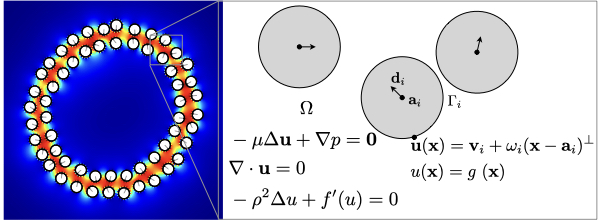
\includegraphics[width=0.45\textwidth]{figures/SpecificAim1/Domain.jpg}
%    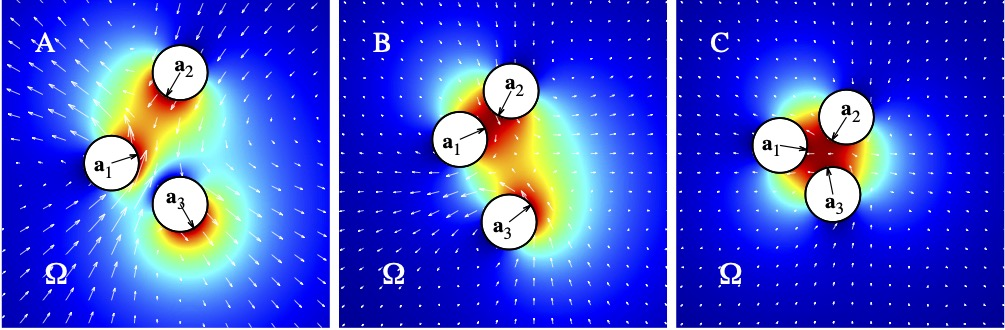
\includegraphics[width=0.45\textwidth]{figures/SpecificAim1/3Particles.jpg}
    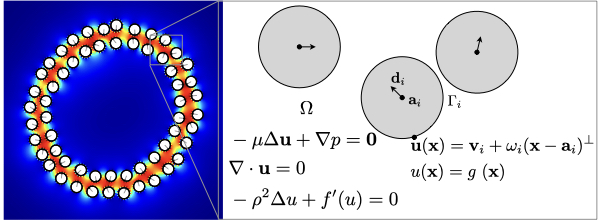
\includegraphics[keepaspectratio,height=2.7cm]{figures/SpecificAim1/Domain.jpg}
    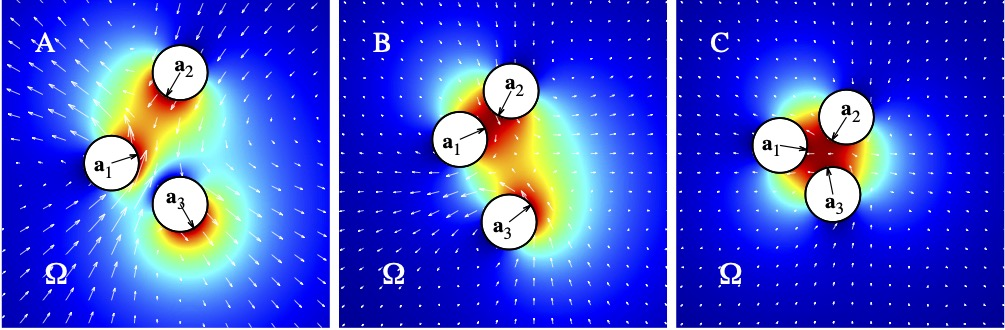
\includegraphics[keepaspectratio,height=2.7cm]{figures/SpecificAim1/3Particles.jpg}
  \end{center}
  \caption{\label{fig:flow_map} \footnotesize {\em Left:} In the HAP
  formulation, a system of exterior problems defines the hydrodynamic
  and hydrophobic interactions. {\em Right:} Particles translate and
  rotate to lower the free energy $F[u]$ subject to \eqref{eq:SL}, $f(u)
  = u^2$, and reach a minimal configuration in panel C. The colormap is
  blue for $u = 0$ and red for $u = 1$. The arrows are the velocity
  field $\mathbf{u}$.}
\end{figure}


\subsection{Problem formulation}
Recently, we have developed a new mathematical model of
self-organization~\cite{FuQuRyYo22,fu-ryh-qua-you2022,Fu2018_SIAM}. The
model takes ideas from the phase field method and leverages boundary
integral equations to speed up computations. To formulate the problem,
consider a collection of $N_b$-many rigid bodies $U_i(t) \subset \mathbb{R}^n$
with boundary $\Gamma_i(t)$.
We call these bodies ``granules''.
The granules are immersed 
in an incompressible, zero-Reynolds number fluid
$\Omega(t) = \RR^n \setminus \cup_{i=1}^{N_b} U_i(t)$
(Figure \ref{fig:flow_map}).

We look for $N_b$-many rigid body transformations
\begin{equation}
\label{eq:RBT}
F_i(\XX,t) = R_i(t)(\XX - \aa_i(0)) + \aa_i(t),\quad \XX \in U_i(0),
\end{equation}
where $i = 1,\ldots,N_b,$
$R_i(t)$ is a rotation (proper orthogonal) $n \times n$ matrix,
$\aa_i(t)$ are the granule centers, and $\XX$ is a reference coordinate.
The transformations \eqref{eq:RBT} tell us how the granules move through space.
Throughout, $\nu$ refers to unit normal pointing into $\Omega(t)$ (Figure \ref{fig:flow_map}).

The key idea is to define the dynamics using the following
boundary value problem system:
\begin{alignat}{4}
  -\mu\Delta \uu + \nabla p &= \mathbf{0}, 
  &&\quad \nabla \cdot \uu = 0, && \quad \xx \in \Omega(t), \label {eqn:stokes} \\
  \label{eqn:phase}
  -\epsilon^2 \Delta \phi + W'(\phi) &= 0, && &&\quad \xx \in \Omega(t),\\
\label{eqn:noslip}        
\frac{dF_i}{dt}(\XX,t) & = \uu(\xx) 
&&=\vv_i + \omega_i \times (\xx - \aa_i), 
&&\quad \xx \in \Gamma_i(t),\\
\label{eqn:material}
\phi(\xx) &= h_i(\XX), &&  &&\quad \xx \in \Gamma_i(t),
\end{alignat}
for $i=1,\ldots,N_b$
and where $\xx = F_i(\XX,t)$.
Finally,
\begin{equation}
\label{eqn:stressbalance}
\int_{\Gamma_i} \left(\sigma  + T_i\right)\nnu \,\dif s = \mathbf{0},\quad
\int_{\Gamma_i} (\xx - \aa_i)\times \left(\sigma + T_i\right) \nnu \,\dif s = \mathbf{0}
\end{equation}
where
\begin{equation}
\label{eqn:hydro_stress}
\sigma = \mu(\nabla \uu + \nabla \uu^T) - pI,\quad 
T_i = \gamma\left[\epsilon^{-1} W'(\phi)I
  + \epsilon\left(\tfrac{1}{2}|\nabla \phi|^2I - \nabla \phi \nabla
  \phi^T\right)\right]
\end{equation}
are the hydrodynamic and phase stresses, respectively; 
$I$ is the $n\times n$ identity matrix.
For vectors $\aa, \bb \in \mathbb{R}^2$,
we follow the usual convention of defining
the ``cross product'' as
$\aa \times \bb = (\aa^{\perp} \cdot \bb) \kk$
where $\kk = (0,0,1) \in \mathbb{R}^3$ and $(a_1,a_2)^{\perp} = (-a_2,a_1)$.

The above form a semi-linear elliptic 
system for evolution of the granules.  Equations~\eqref{eqn:stokes} are the
Stokes equations that describes the velocity $\uu$ and pressure $p$ of
the aqueous region with viscosity $\mu$.  Equation~\eqref{eqn:phase} describes the
phase transitions of the scalar order parameter $\phi$ with a decay
length $\epsilon$.
The scalar function $W(\phi)$ is a well potential where the local 
minimima representing low energy states of the water phase.
Mathematically, this order parameter is responsible for
the attraction and adhesion between granules that want to align boundaries
of like phase.

The next three equations are the moving domain boundary conditions.
Equations~\eqref{eqn:noslip} specify a no-slip
boundary condition for a rigid body with translation velocity $\aa'_i(t) = \vv_i$
and angular velocity $\omega_i$
about the point $\aa_i(t) \in U_i(t)$.
($\omega_i$ is the axial vector of the
skew symmetric matrix $R'_i(t)$.)
In
equation~\eqref{eqn:material}, the function $h_i$ is a material label
specifying the phases at water-granule interface.
The boundary condition for $\phi$ is transported by the flow
and satisfies $\phi_t + \uu \cdot \nabla \phi = 0$ on $\Gamma_i$.
Finally,
equation~\eqref{eqn:stressbalance} closes the system by
requiring that the force and torque generated by 
hydrodynamic stress balances that generated by phase stress $T_i$ in
\eqref{eqn:hydro_stress}.
The parameter $\gamma > 0$ is surface tension. 

We call the rigid bodies $U_i(t)$ granules since they are small, compact
parcels of a suspended media, e.g. lipids, Janus spheres.
We use the shape and boundary conditions for $U_i$ to capture the local
properties of the suspended media. 
We have departed from the terminology ``particles'' here
to emphasize the role played by their finite size. 
In our simulations (see section \ref{sec:specific_aim1}),
we include a finite length repulsion to avoid particle
collisions.




The system~\eqref{eq:RBT}--\eqref{eqn:stressbalance}
has the energy law
\begin{equation}
\label{eq:energy_law}
  \frac{d}{dt}E
  = - \int_{\Omega_t}\tfrac{1}{2}\mu|\nabla \uu + \nabla
  \uu^T|^2 \,d\xx,\quad
    E = \gamma \int_{\Omega(t)}
  \frac{\epsilon}{2} |\nabla \phi|^2 + \frac{1}{\epsilon} W(\phi) \,d\xx.
\end{equation}
Here $E$ is the energy stored in the phase transitions.
Mathematically, the energy law states that changes
in granule configuration instantaneously change the phase energy $E$.
The dynamics are such that the change energy
is lost due to hydrodynamic dissipation.
Further details and generalizations are provided in
the Specific Aim 1 section \ref{sec:specific_aim1}.

Because $E$ depends both on $\phi$ and $\Omega(t)$,
the derivation of \eqref{eq:energy_law}
is somewhat subtle and has been worked out in detail in \cite{Fu2018_SIAM}.
It goes as follows.
Using the Rayleigh Transport Theorem, 
the time derivative out $E$ yields an energy
density flux involving the phase stress $T_i$
at the boundary, plus a bulk term involving 
the Euler-Lagrange derivative of $E.$
The Euler-Lagrange derivative vanishes due to~\eqref{eqn:phase}
and the boundary flux transforms into viscous dissipation due to 
\eqref{eqn:hydro_stress} and the Stokes equations. 


In terms of physical justification, the
derivation of the one-dimensional version of our model
was carried out by \cite{MaRa76} and \cite{ErLjCl89}
using a Landau expansion of the
free energy density for a single-well potential.
The double-well potential case was derived by
Gompper in \cite{GoHaKo94} to describe metastable coordination of water.
In the field of surface chemistry \cite{Israelachvili1954},
there is a large empirical literature on properties of
long-range hydrophobic interaction~\cite{LeRaPa77,KoNa15,
Nagle17,Lum1999, Lin2005, Meyer2006, Ducker2016,Jackson2016,Gletal88,Aketal17,Ch05}.
The stress~\eqref{eqn:stressbalance} was first
identified by PIs Ryham and Young in~\cite{Fu2018_SIAM}
and generalizes one-dimensional hydrophobic interaction to
the $n$-dimensional setting. 

Finally, we mention that in the single-well case
$W(\phi) = \tfrac{1}{2}u^2,$ \eqref{eqn:phase} takes the form
of a screened Laplace (SL) equation $-\epsilon^2 \Delta \phi + \phi =0$.
If the material label $h_i = 1$ everywhere, then $\phi$
has a boundary layer going from $1$ at the boundary to $0$ in the bulk
and one can prove that 
\begin{equation}
\label{eqn:math_motivation}
\lim_{\epsilon \to 0} E = \frac{\gamma}{2} \int_{\partial \Omega} 1 \,dS
\end{equation}
under the assumption that $\Omega$ has a class $\mathbf{C}^2$ boundary \cite{}.
In other words, the phase energy can be viewed as an
approximation of surface energy that ``extends'' into the bulk.
In the general case, $h_i^2$ replaces $1$ in \eqref{eqn:math_motivation}.
We are confident that \eqref{eq:RBT}--\eqref{eqn:stressbalance}
is a correct description of long-range surface interactions.

The model has a broad range of applicability to self-organization
phenomena in chemistry and biological physics. For one,
the formulation~\eqref{eq:RBT}--\eqref{eqn:stressbalance} captures
exactly the right behavior expected from amphiphilic self-assembly.
For example, three bodies with amphiphilic label
(see section \ref{sec:specific_aim1}) spontaneously
self-organize to sequester the hydrophobic fluid phase
(the red phase in Figure \ref{fig:flow_map}).
Moreover, a simple change of boundary conditions from
amphiphilic, to biased hydrophobic, to polar results in distinct
equilibrium morphologies (Figure~\ref{fig:self-assembly2}).
Since the formulation is
scale independent, it can represent a suspension of amphiphiles, where
the granules represent the mean properties of a small collection of
lipids, at the nanoscopic scale. For larger scales, the representation
is literal and the granules Janus spheres. The proposal deals with the
physical origins in section ().
\todo[inline]{
List applications; don't forget Bertozzi.}

\begin{figure}[t!]
  \begin{center}
    \begin{tabular}{m{0.1cm}m{1.8in}m{1.8in}m{1.8in}}            
      (a)
    &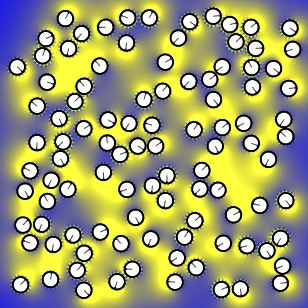
\includegraphics[width=1.8in]{figures/SpecificAim1/N100B1.jpg}
    &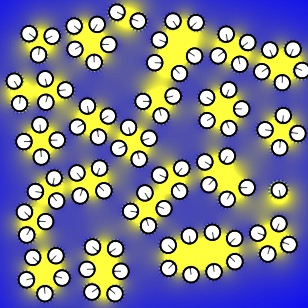
\includegraphics[width=1.8in]{figures/SpecificAim1/N100B2.jpg}
     &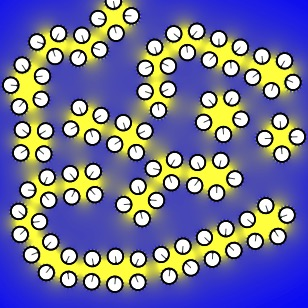
\includegraphics[width=1.8in]{figures/SpecificAim1/N100B3.jpg}    \\
     (b)
    &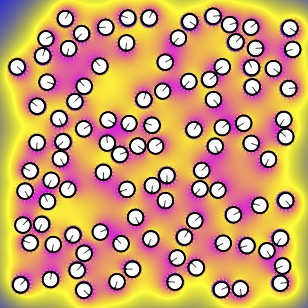
\includegraphics[width=1.8in]{figures/SpecificAim1/N100C1.jpg}
    &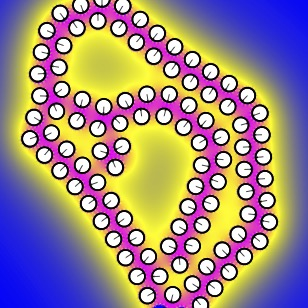
\includegraphics[width=1.8in]{figures/SpecificAim1/N100C2.jpg}
      &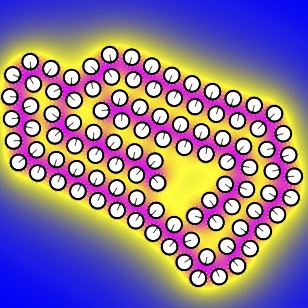
\includegraphics[width=1.8in]{figures/SpecificAim1/N100C3.jpg}    \\
    (c)
      &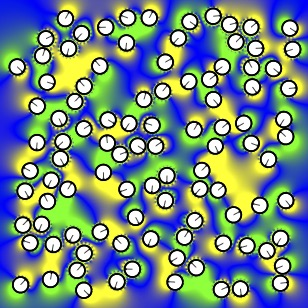
\includegraphics[width=1.8in]{figures/SpecificAim1/N100A1.jpg}
      &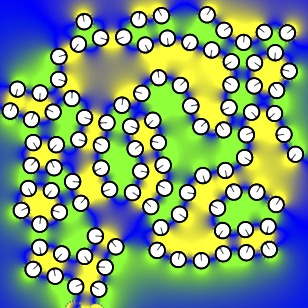
\includegraphics[width=1.8in]{figures/SpecificAim1/N100A2.jpg}
      &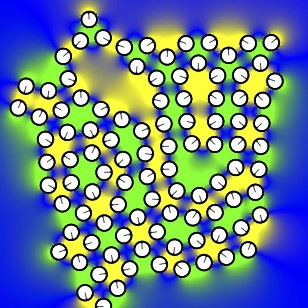
\includegraphics[width=1.8in]{figures/SpecificAim1/N100A3.jpg}    \\
      &\multicolumn{1}{c}{$t = 0$}
      &\multicolumn{1}{c}{intermediate time}
      &\multicolumn{1}{c}{long time}
  \end{tabular}
  \end{center}
  \vspace{-20pt}
  \caption{\footnotesize \label{fig:self-assembly2} Rows (a)-(c) have
  the same initial configuration but different boundary conditions $g$.
  In row (a), self-assembly with an amphiphilic boundary condition
  results in a bilayer pattern shielding the hydrophobic core (yellow,
  $u > 0$) from the aqueous phase (blue, $u = 0$). Row (b) shows
  particles with a hydrophobic intensity that is greater on one side of
  the particle (magenta) than the other (yellow). In row (c), green is
  for $u < 0$, yellow is for $u > 0$, and blue is for $u = 0$. Particles
  orient like sides to form a checkerboard pattern.}
\end{figure}

\begin{figure}[t!]
\begin{center}
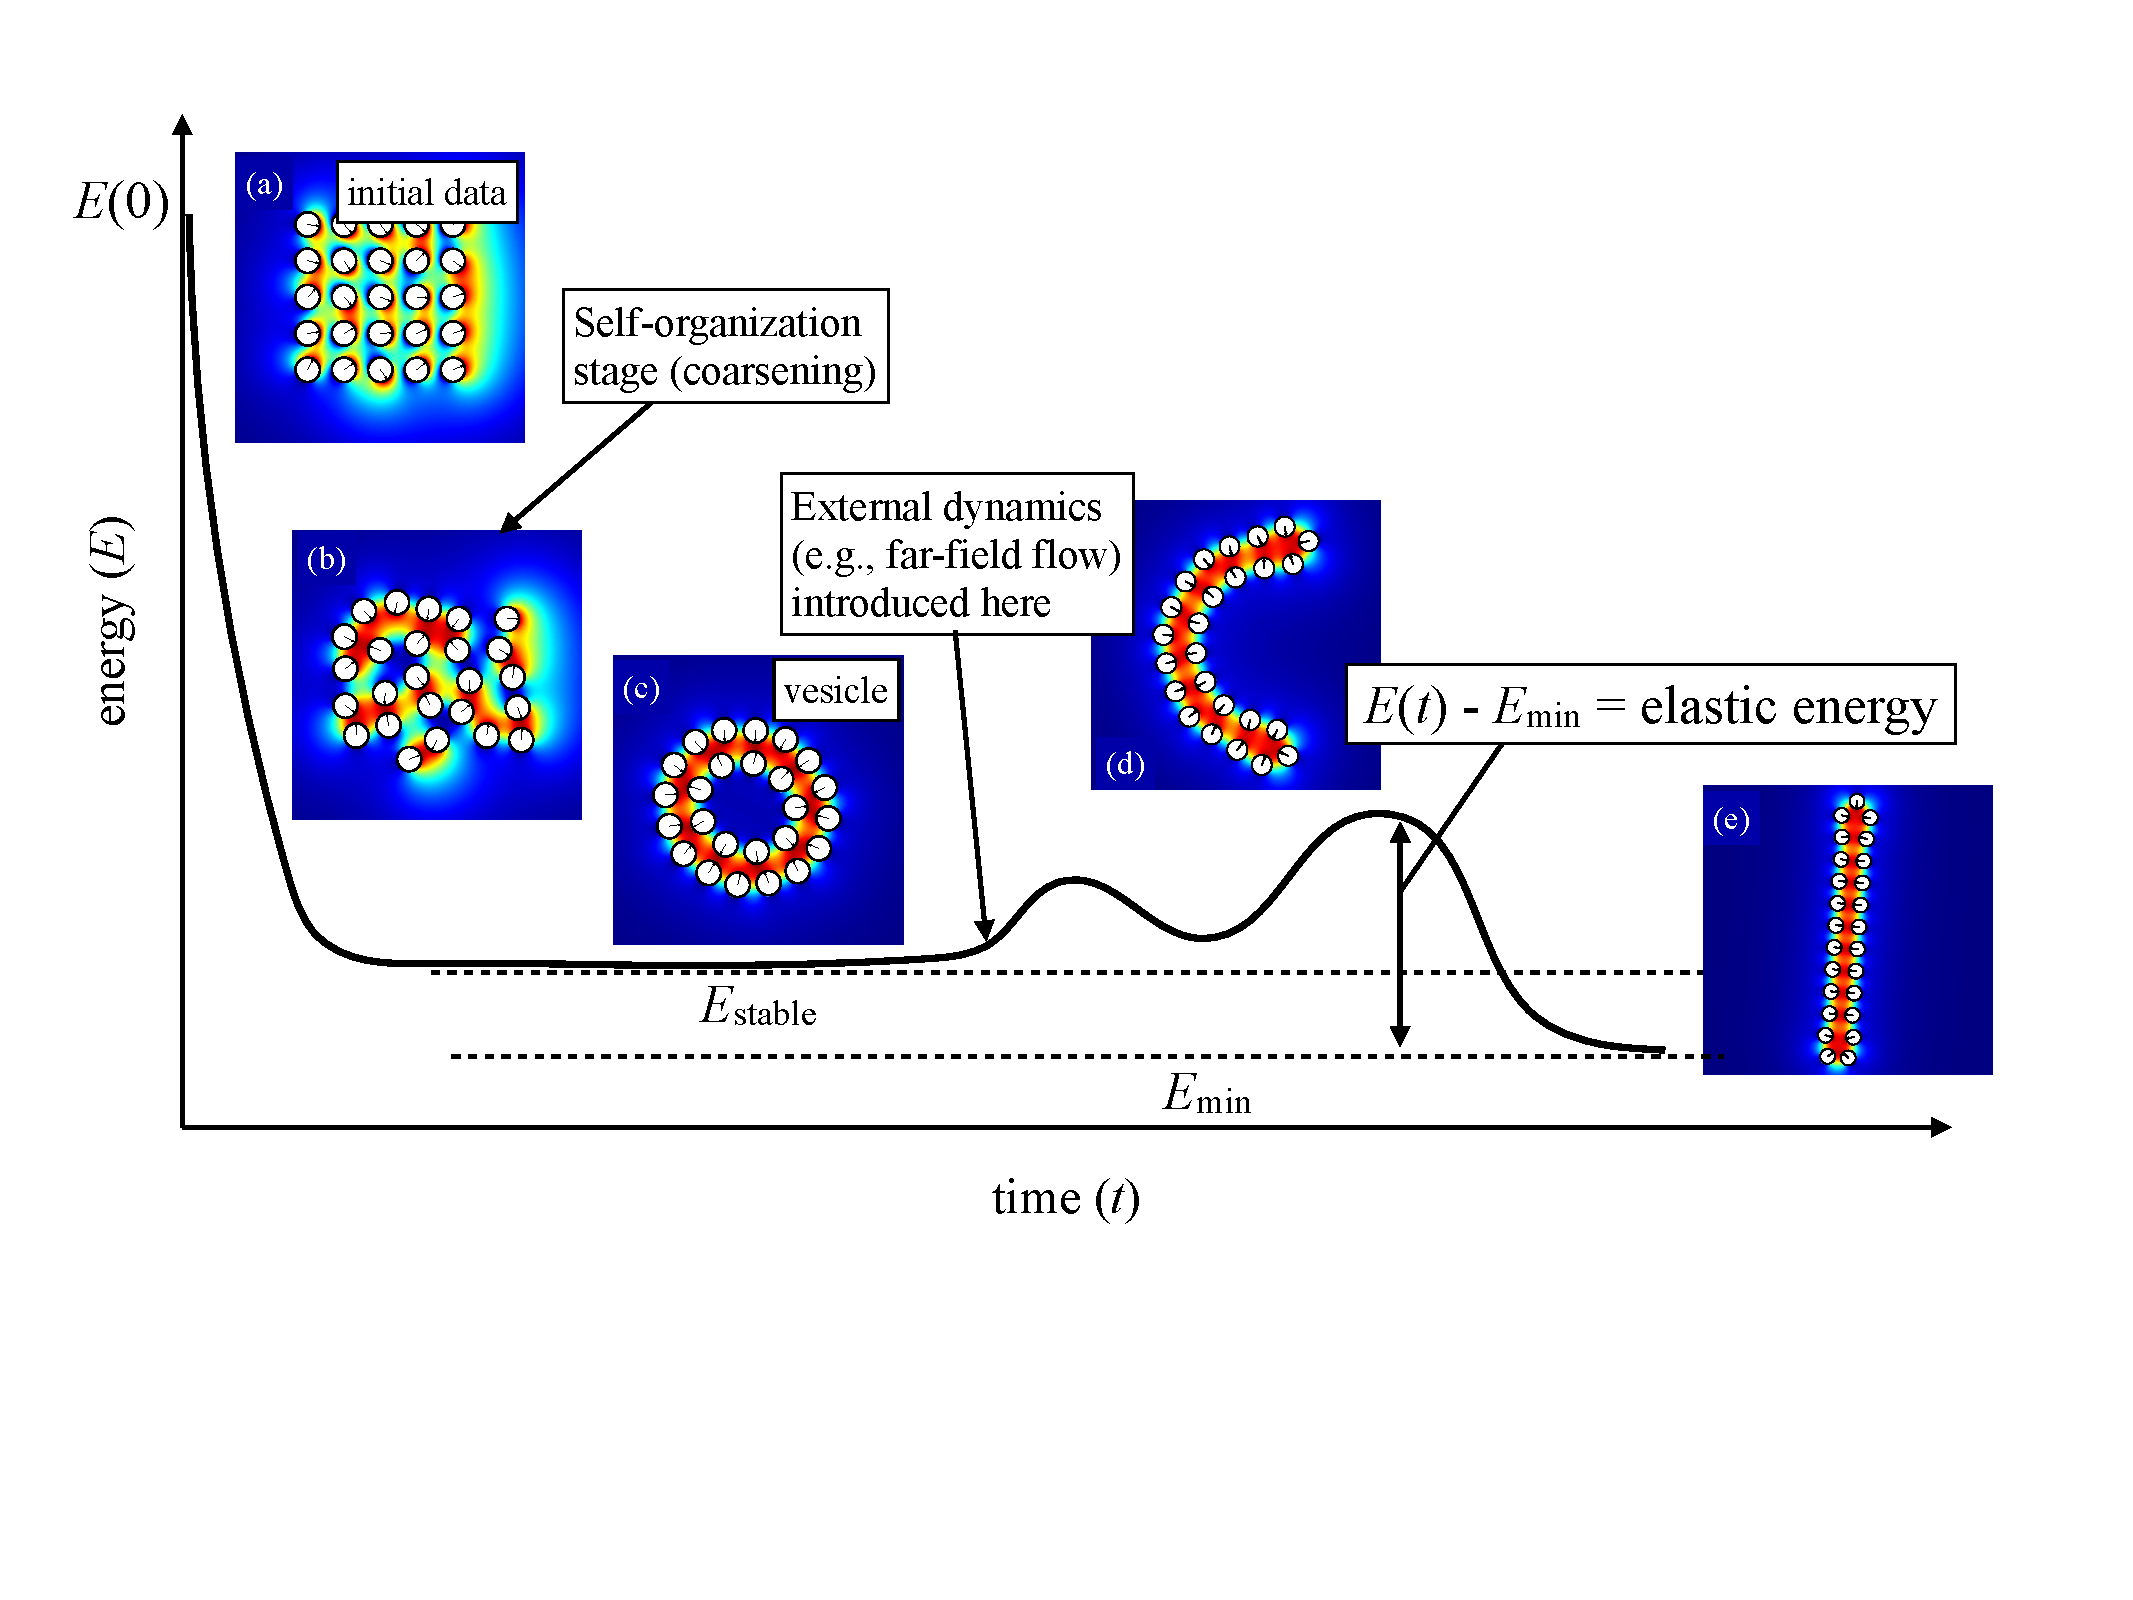
\includegraphics[width=\textwidth]{figures/Background/coarsening.pdf}
\end{center}
\caption{\label{fig:coarsening}}
\end{figure}
%%%%%%%%%%%%%%%%%%%%%%%%%%%%%%%%%%%%%%%%%%%%%%%%%%%%%%%%%%%%%%%%%%%%%%%%%%%%%%%%%%%%%%%%%%
\subsection{Boundary integral formulation}
\label{sec:bie}

\begin{wrapfigure}[10]{r}{2in}
  \todo[inline]{A figure comparing FEM versus BIE meshes}
  \caption{\label{fig:fem_vs_bie} \footnotesize A finite element method
  requires meshing the entire domain (typically into triangles), while a
  BIE only requires meshing the boundary of the domain.}
\end{wrapfigure}
Boundary integral equations (BIEs) are a reformulation of elliptic PDEs
including the Stokes equation~\eqref{eqn:stokes} and the phase
equation~\eqref{eqn:phase} in the special case of $f(u) =
\tfrac{1}{2}u^2$. Using the Stokes equation as an example, its solution
can be written as a convolution 
\begin{align*}
  \uu(\xx) = \int_{\partial\Omega_t} G(\xx - \yy) \ssigma(\yy) \, ds_\yy,
\end{align*}
where $G(\xx - \yy)$ is a carefully chosen derivative of the PDE's
fundamental solution and $\ssigma: \partial \Omega_t \rightarrow \RR^2$
is an unknown density function. The BIE reformulation has several
immediate advantages including a dimension reduction since $\ssigma$ is
defined only on $\partial \Omega_t$, and the far field boundary
condition of the PDE is automatically satisfied. The density
function $\ssigma$ is chosen to satisfy the boundary condition, and this
results in a BIE 
\begin{align*}
  \gg(\xx) = \lambda \ssigma(\xx) + 
    \int_{\partial\Omega_t} G(\xx - \yy) \ssigma(\yy) \, ds_\yy,
    \quad \xx \in \partial\Omega_t,
\end{align*}
where $\gg$ is the Dirichlet boundary condition, and $\lambda$ is a
constant that depends on the choice of $G$. For numerical stability,
choices of $G$ that result in second-kind Fredholm integral equations,
meaning $\lambda \neq 0$, are preferred.

A consequence of the dimension reduction in a BIE formulation is that
complex geometries are much easier to resolve than a mesh-based method
since only $\partial \Omega_t$ needs to be discretized
(Figure~\ref{fig:fem_vs_bie}). Additional advantages of a BIE
formulation includes a discretization that is high-order, or even
spectrally, accurate; results in a well-conditioned linear system that
can be solved iteratively with a mesh-independent number of iterations
of a Krylov method such as the generalized minimal residual method
(GMRES). However, BIEs do have several challenges: nearly touching
granules requires a quadrature rule for nearly-singular integrals; their
discretization results in dense matrices; and they cannot immediately be
applied to non-linear PDEs. The BIE community, including PI Quaife, has
developed a variety of tools to address these numerical challenges, and
we discuss our planned approach in Section~\ref{sec:specificaim2}.




\subsection{Outline of the proposal}
